\documentclass[12pt,a4paper]{article}
\usepackage[utf8]{inputenc}
\usepackage{graphicx}
\graphicspath{{graphics/}}
\DeclareGraphicsExtensions{.pdf,.jpeg,.jpg,.png}

\usepackage{amsmath} % equations
\usepackage{fancyhdr} % nicer page header

\setlength{\parindent}{0pt} % no paragraph indents
\setlength{\parskip}{1em} % paragraphs separated by one line

\newcommand\experiment{N-Body Simulations with REBOUND} %%%%% experiment name
\newcommand\groupno{Group 3+10}       %%%%% group number
\newcommand\names{Pratyush Singh,\\
                  Proshmit Dasputpa,\\
                  Erasyl Telman}        %%%%% full names
\newcommand\expdate{07/03/2025}    %%%%% date of experiment day

\begin{document}
\begin{titlepage}
   \begin{center}
        \vspace*{3cm}
        \Huge{\experiment}
				
        \vspace{0.5cm}
        \LARGE{Lab course protocol}
				
        \vspace{3 cm}
        \Large{\groupno}
				
        \vspace{0.25cm}
        \large{\names}
				
        \vspace{2 cm}
        \Large{\expdate}
				
        \vspace{0.25 cm}
        \Large{Advanced lab course in astronomy\\
				Eberhard Karls Universit\"at T\"ubingen}
				
				\vspace{0.1 cm}
        \Large{WiSe 2024/25}
				
       \vfill
    \end{center}
\end{titlepage}

\pagestyle{fancy}
\fancyhf{}
\setlength{\headheight}{14.5pt}
\lhead{\groupno; \experiment}

\section*{Abstract}
This is optional, but never longer than half a page.

\tableofcontents
\newpage

\setcounter{page}{1}
\pagestyle{fancy}
\fancyhf{}
\rhead{\thepage}
\lhead{\groupno; \experiment}

\section{Introduction}\label{sec:intro} % labels allow references, particularly important for figures and tables
Very short summary what the experiment is about and why the subject plays a role in astronomy/astrophysics.

\section{Theory}\label{sec:theory}
\subsection{Classical N-Body Problem}
\subsection{Time Integrators}
\subsubsection{Leapfrog}
\subsubsection{IAS15}
\subsubsection{WHFast}
\subsubsection{Gragg-Bulirsch-Stoer}
% A short overview over the most important points of the experiment, including the answers
% to the questions (2 to 3 pages maximum plus questions).

% \begin{equation}\label{eq:H}
%      \hat{H} \psi = i \hbar \frac{\partial \Psi}{\partial t}
% \end{equation}

% \begin{align}
%      \frac{D}{D_0} &= e^{-\frac{\mu}{\rho}\rho x} \\
%     ln\left(\frac{D}{D_0}\right) &= -\frac{\mu}{\rho}\rho x \\
%     x &= \frac{-ln\left(\frac{D}{D_0}\right)}{\frac{\mu}{\rho}\rho}
% \end{align}
\subsection{REBOUND}

\section{Experiment}
\subsection{Two Body Problem}
\subsection{Three Body Problem and Stability of the Planet System}
\subsection{Jupiter and Kirkwood Gaps}
\subsection{Resonant Capture of a Planet}
% For each experimental part:
% \begin{enumerate}
%  \item Description of setup and procedure (1 to 3 sentences each).
%  \item Tabulated measurement results.
%  \item Analysis and graphs (including detailed calculation, giving all
% formulae and values with units used).
%  \item Discussion of result (1 to 3 sentences).
% \end{enumerate}

% \subsection{Subsection}
% You might use subsections \dots

% \subsubsection{Subsubsection}
% \dots but not more than two layers.

% And please reference all figures and tables in the text, like Figure~\ref{fig:mcp} and Table~\ref{tab:ex}.

% \begin{figure}[t]
% \centering
% 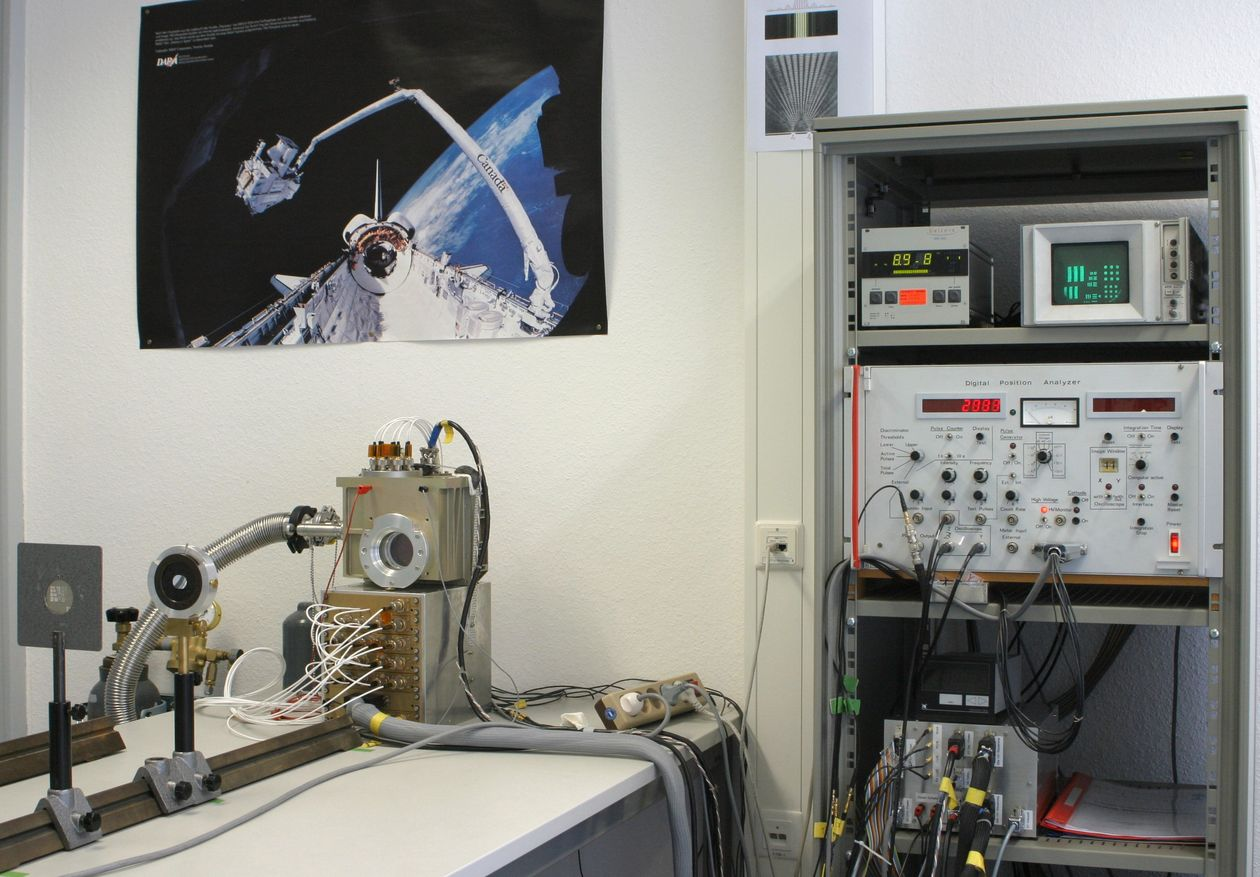
\includegraphics[width=.8\textwidth]{MCP-lab.jpg}
% \caption{All figures need a caption below. The caption should describe the figure and highlight important aspects, the rest is written in the main text. Each figure needs a reference in the text! If you are not the creator of the figure, put the appropriate citation in the caption}
% \label{fig:mcp}
% \end{figure}

% \begin{table}[t]
% 	\centering
% 	\caption{All tables need a caption above. The caption should describe the table and highlight important aspects, the rest is written in the main text. Each table needs a reference in the text! Units are given in the column headers.}
% 	\label{tab:ex}
% 	\begin{tabular}{cccc}
% 		\hline\noalign{\smallskip}
% 		Beam energy & $\Phi_\mathrm{nom}$ & $\Phi_\mathrm{app,HR}$ & $\Phi_\mathrm{app,AR}$ \\
% 		(keV) &  ($\mathrm{cm^2}$) & ($\mathrm{cm^2}$) & ($\mathrm{cm^2}$) \\
% 		\noalign{\smallskip}\hline\noalign{\smallskip}
% 		150  & $3.4 \cdot 10^{10}$ & $3.5 \cdot 10^{10}$ & $3.4 \cdot 10^{10}$ \\
% 		150  & $1.7 \cdot 10^{11}$ & $1.7 \cdot 10^{11}$ & $1.7 \cdot 10^{11}$ \\
% 		1400 & $7.5 \cdot 10^{8}$  & $9.9 \cdot 10^{8}$  & $7.4 \cdot 10^{8}$  \\
% 		\noalign{\smallskip}\hline
% 	\end{tabular}
% \end{table}

% Put also citations in the text wherever necessary and appropriate. Citations are to be used whenever external material is included, also in the text \cite{basic-contrib}, \cite{basic-online}, \cite{basic-DOI}, \cite{basic-journal}, \cite{basic-mono}.

\section{Conclusions}
An important section in which you should critically review the experiment and its results. Mention also parts that did not work out as expected, but keep a neutral to positive view. This can span from a few sentences to half a page.

\setcounter{secnumdepth}{0}
\begin{thebibliography}{99.}
% Book Chapter
\bibitem{basic-contrib} Brown B, Aaron M (2001) The politics of nature. In: Smith J (ed) The rise of modern genomics, 3rd edn. Wiley, New York, p 234--295  
%
% Online Document
\bibitem{basic-online} Dod J (1999) Effective Substances. In: The dictionary of substances and their effects. Royal Society of Chemistry. Available via DIALOG. \\
http://www.rsc.org/dose/title of subordinate document. Cited 15 Jan 1999
%
% Journal article by DOI
\bibitem{basic-DOI} Slifka MK, Whitton JL (2000) Clinical implications of dysregulated cytokine production. J Mol Med, doi: 10.1007/s001090000086
%
% Journal article
\bibitem{basic-journal} Smith J, Jones M Jr, Houghton L et al (1999) Future of health insurance. N Engl J Med 965:325--329
%
% Monograph
\bibitem{basic-mono} South J, Blass B (2001) The future of modern genomics. Blackwell, London 
%
\end{thebibliography}
\appendix
\section{Appendix}
\subsection{Code}
Please attach here your original handwritten notes and other documents created during the experiment.

\end{document}

